\documentclass[11pt]{article}
\usepackage[margin=0.9in]{geometry}
\usepackage{amsmath,amssymb,booktabs,graphicx}
\usepackage[hidelinks]{hyperref}
\newcommand{\Tr}{\operatorname{Tr}}
\newcommand{\eps}{\epsilon}
\title{Protection, mitigation, and algorithm choice for Hubbard dynamics\\
\large Analytical forms and first resource curves}
\author{Working research note}
\date{22 September 2026}
\begin{document}
\maketitle

We compare physical-qubit computation with probabilistic error cancellation
(PEC), partially protected STAR computation, and full surface-code fault
tolerance on a common qubit array. We first expose the analytical dependence
on problem size, evolution time, and circuit refinement. The figures evaluate
declared reference models; they do not establish crossover locations for a
compiled device. Circuit compilation with CUDA-Q Logical comes next, followed
by Trotter-error calibration. Qubitization is a subsequent algorithm comparison.

\section{Task, precision, and the shared circuit}
We take an even, open $L\times L$ square with $N=L^2$ Hubbard sites,
$2N$ fermionic modes, and
\begin{equation}
 H/J=-\sum_{\langle ij\rangle,\sigma}
 (c^\dagger_{i\sigma}c_{j\sigma}+\mathrm{h.c.})
 +u\sum_i n_{i\uparrow}n_{i\downarrow},\qquad u=U/J=4.
\end{equation}
The initial state is the half-filled N\'eel product state. We estimate the
central-site doublon expectation $D=\langle n_{i\uparrow}n_{i\downarrow}\rangle$
at dimensionless time $\tau=Jt/\hbar$. The physical device has $Q=M^2$ qubits,
nearest-neighbor gates of duration $10$~ns, measurement and reset of $100$~ns
each, and physical error parameter $p=10^{-3}$.

The requested accuracy is $\eps=\eta |D|$, with $\eta=0.01$ and failure
probability $\delta=0.05$. Since the first resource curves precede dynamics
calculations, we display them at a declared reference $D_*=0.1$, giving
$\eps=10^{-3}$, and retain $D_*$ as a sensitivity. This is a conditional
resource estimate, not a prediction of the doublon curve. Strict relative
error at $D=0$ needs separate treatment; we do not introduce an implicit
absolute floor. A production estimator would need a pilot or sequential
confidence procedure if $D$ is unknown.

Campbell's phase-estimation calculation uses an additive total-energy error
$0.0051L^2$, approximately a fixed relative energy tolerance~\cite{campbell}.
This is equivalent to fixed additive accuracy in energy per site. Our $D$
is already intensive: fixing its absolute error does not itself impose an
increasing precision penalty with $N$. Relative error is nevertheless a useful
choice when the size of the physical signal is the relevant target.

We reserve fractions $(0.5,0.25,0.1,0.075,0.075)$ of $\eps$ for statistical,
Trotter, logical-fault, synthesis, and magic-state error, respectively. Unused
fractions are not reallocated in this first comparison. PEC channel knowledge
is idealized, with zero residual mitigation bias; SPAM is included in the
physical PEC reference. No spatial truncation is made. These choices leave a
clear place for calibration, truncation, and mitigation-bias costs later.

We hold the same step count $r$ across architectures, initially
$r=\lceil\rho\tau\rceil$, $\rho=4$. This is a circuit family, not an assertion
that its Trotter bias meets the reserved budget. Within each decomposition,
the ideal algorithmic error is common to all three architectures. The cost
response to changing $r$ is not common.

\subsection{Termwise second order}
In a fixed-number sector, the single-$Z$ terms of the onsite interaction are
a known phase. With $E=2L(L-1)$ spatial bonds, the remaining Jordan--Wigner
Hamiltonian has
\begin{equation}
 K=4E+N=9N-8L,\qquad
 \lambda=\sum_\ell |h_\ell|=2E+\frac{|u|N}{4}=5N-4L.
\end{equation}
There are four hopping Pauli strings per spatial bond, each with coefficient
magnitude $1/2$, and one onsite $ZZ$ per site, with magnitude $|u|/4$.
Our convention is $U_P(\theta)=e^{-i\theta P}$; thus $R_z(\phi)$ has
$\phi=2\theta$, and a $T$ gate has $|\theta|=\pi/8$ up to a global phase.

For a symmetric product over the $K$ terms, choose onsite terms at both ends
of the ordering and merge adjacent identical rotations at the center and
between steps. Before further commuting or Clifford simplifications,
\begin{equation}\label{eq:termwise}
 R_{\rm term}=r(2K-2)+1,\qquad \Theta_{\rm term}=\tau\lambda.
\end{equation}
The count follows from $r(2K-1)$ rotations after center merging and $r-1$
additional boundary merges. Every coefficient has total positive duration
$\tau$, proving the angle identity. Signed higher-order stages instead
multiply the angle sum by their total absolute stage weight. The histogram,
not merely $\Theta$, is retained for channel evaluation.

\subsection{Campbell plaquette second order with open boundaries}
Campbell partitions hopping into disjoint pink and gold tiles and applies
\begin{equation}\label{eq:plaq}
 S_2(\Delta)=e^{-i\Delta H_I/2}e^{-i\Delta H_p/2}
 e^{-i\Delta H_g}e^{-i\Delta H_p/2}e^{-i\Delta H_I/2},
 \qquad \Delta=\tau/r.
\end{equation}
We adapt the periodic construction to open boundaries. The pink partition
has $P=L^2/4$ complete plaquettes. The shifted gold partition has
$G=(L/2-1)^2$ complete plaquettes and $B=2(L-2)$ isolated boundary bonds.
Each bond belongs to exactly one partition, since $4(P+G)+B=E$.

A single-spin four-site hopping cycle has eigenvalues $\{2,0,0,-2\}$.
Campbell's circuit implements its evolution with two variable-angle Pauli
rotations and eight fixed $T$ gates~\cite[Appendix E.1]{campbell}. An isolated
bond needs two commuting hopping Pauli rotations per spin. For $L\geq4$,
including both spin species and exact onsite boundary merging, this gives
\begin{align}
 R_{\rm plaq}&=N(r+1)+4r(2P+G+B),\\
 T_{\rm fixed}&=16r(2P+G),\\
 \Theta_{\rm dyn}&=\tau\left[\frac{|u|N}{4}+4(P+G)+2B\right].\label{eq:plaqangle}
\end{align}
For $L=2$ the gold partition is empty: the two pink half steps merge, so
$2P$ becomes $P$ in the count formulas. The angle formula is unchanged.
At $L=4$, $\tau=1$, $r=4$, these formulas give
$(R_{\rm plaq},T_{\rm fixed},\Theta_{\rm dyn})=(288,576,44)$.

The compiled total angle includes $T_{\rm fixed}\pi/8$. Consequently, the
invariance of $\tau\lambda$ under refinement in Eq.~\eqref{eq:termwise}
does not apply to all non-Clifford operations in Eq.~\eqref{eq:plaq}.
The fixed basis changes are an algorithm-dependent STAR exposure even when
the variable rotations have no injection floor. Distilling those fixed
angles is an immediate hybrid candidate. Hamming-weight phasing, cancellations
between neighboring basis changes, and angle extraction are later compiler
optimizations. Campbell neglects fermionic-swap Clifford costs in his
non-Clifford metric; our eventual nearest-neighbor accounting must restore them.

\section{Sampling and the one-week constraint}
Write a PEC inverse as $\mathcal{E}^{-1}=\sum_a c_a\mathcal{P}_a$, with
$\gamma=\sum_a|c_a|$. For a circuit of independently cancelled channels,
$\Gamma=\prod_j\gamma_j$. Using the centered observable $D_i-I/2$, the
signed, rescaled single-shot estimator lies in $[-\Gamma/2,\Gamma/2]$.
Hoeffding's inequality therefore gives the sufficient statistical sample count
\begin{equation}\label{eq:shots}
 n\geq \frac{\Gamma^2}{2\eps_{\rm stat}^2}\log\frac{2}{\delta},
 \qquad N_0=\left\lceil\frac{\log(2/\delta)}{2\eps_{\rm stat}^2}\right\rceil.
\end{equation}
The implementation uses $N_0\Gamma^2$, with final shot rounding negligible
on these scales. At the default precision $N_0=7{,}377{,}759$.
This bounded-sample reference is more conservative than a Gaussian interval
using an assumed Bernoulli variance. It is common across arms and can be replaced
without changing their exposure laws. PEC follows the standard inverse-channel
construction~\cite{temme}; its ideal implementation and exact channel knowledge
are assumptions of these curves.

For whole-circuit acceptance $a$, attempt time $t_a$, and
$m=\lfloor Q/Q_{\rm copy}\rfloor$ independent replicas,
\begin{equation}\label{eq:time}
 T_{\rm answer}\simeq\frac{N_0\Gamma^2 t_a}{am},\qquad
 Q_{\min}^{\rm area}\simeq Q_{\rm copy}
 \left\lceil\frac{N_0\Gamma^2t_a}{aB_{\rm week}}\right\rceil,
 \quad B_{\rm week}=604800~\mathrm{s}.
\end{equation}
At least one copy is required. A circuit longer than the cutoff is infeasible
regardless of replication. These equations use area packing, not a demonstrated
placement on the square device. Integer-square rounding and routing footprints
belong to the compilation refinement. The figures set $a=1$; resource-state
rejection belongs in $t_a$, not in whole-circuit acceptance. Setup and calibration
time are not yet modeled.

Writing $\chi=\log\Gamma^2$, the mitigation wall is
\begin{equation}
 \chi\lesssim\log\frac{a m B_{\rm week}}{N_0t_a}.
\end{equation}
Budget and replicas therefore buy logarithmic exposure under this model.
This is a property of the specified estimator, not an impossibility claim
about all physical-qubit strategies.

\section{Physical-qubit reference}
For $k$ qubits, let $K_p=4^k$ and let total depolarizing error probability $p_k$
mean a uniformly random nonidentity Pauli. The channel has nonidentity Pauli
eigenvalue $s=1-K_pp_k/(K_p-1)$. Its inverse has identity coefficient
$1+p_k/s$ and $K_p-1$ coefficients $-p_k/[(K_p-1)s]$, hence
\begin{equation}
 \gamma_{\rm dep}=1+\frac{2p_k}{s},\qquad
 \log\gamma_{\rm dep}^2=4p_k+O(p_k^2).
\end{equation}
A binary Pauli-flip channel has $\gamma_{\rm flip}=1/(1-2p)$.
We sum the exact logarithms over two-qubit gates ($p$), single-qubit gates
($p/10$), idle layers ($p$), preparation flips ($p$), and the two measured
observable bits ($p$). This implements the accepted per-layer idle convention.
With perfect virtual Pauli corrections, the leading dependence is
\begin{equation}
 \chi_{\rm phys}\simeq4pG_2+4(p/10)G_1+4pG_{\rm idle}+4pG_{\rm SPAM}.
\end{equation}

For the initial figure only, use the explicit workload proxies
\begin{align}
 G_2&=2R+T_{\rm fixed},&G_1&=5R+T_{\rm fixed},\\
 D_g&=\left\lceil1.25\frac{2G_2+G_1}{2N}\right\rceil,&
 G_{\rm idle}&=2ND_g-2G_2-G_1,\\
 t_a&=t_{\rm reset}+(D_g+1)t_g+t_{\rm meas},&Q_{\rm copy}&=2N.
\end{align}
The N\'eel preparation adds $N$ noisy $X$ gates in one layer, plus $2N$
preparation flips; only the final two observable bits require readout.
The coefficients above are declared placeholders for local compilation and
occupancy, not gate counts imported from a paper. They do not implement the
planned snake Jordan--Wigner routing. In particular, the first figure is not
a physical nearest-neighbor feasibility claim. Replacing these coefficients
by compiled $G_2$, $G_1$, depth, and idle volume is the next high-priority step.
Symmetry selection, local PEC, and learned mitigation are separate later
strategies with their own bias and acceptance evidence.

\section{STAR exposure and protection}
For an independent residual dephasing probability $q_j$,
\begin{equation}\label{eq:star}
 \Gamma^2=\prod_j(1-2q_j)^{-2},\qquad
 \chi=-2\sum_j\log(1-2q_j)\simeq4\sum_jq_j.
\end{equation}
We evaluate three reference models. Original STAR has
$q_j=q_0=4p/15$ after repeat-until-success (RUS), giving
$\chi\simeq(16p/15)(R+T_{\rm fixed})$~\cite{akahoshi}.
The small-angle model uses $q_j=\alpha p|\theta_j|$, with
$\alpha=1.5$ in our angle convention~\cite{toshio}. A third curve adds a
variable-rotation floor $f=10^{-5}$, motivated by injection and code growth
but not fitted at our operating point~\cite{chung}.

For both small-angle curves, fixed $T$ gates use the original injection
channel $q_0$. We do not extrapolate the small-angle coefficient to fixed
$\pi/8$ rotations. Thus their leading exposure is
\begin{equation}\label{eq:starcompiled}
 \chi_{\rm STAR}\simeq4\alpha p\Theta_{\rm dyn}+4fR
       +\frac{16p}{15}T_{\rm fixed}.
\end{equation}
Each term names a distinct possible limitation. The floor competes with the
angle term when $fR\sim\alpha p\Theta_{\rm dyn}$. The basis-change term can
also dominate. The code evaluates Eq.~\eqref{eq:star}, retaining the small
$O(\sum_jq_j^2)$ dependence on angle splitting. The channel laws remain
leading-order physical approximations, even when the product is evaluated
without an exponential approximation.

Both encoded arms use the same per-patch, per-cycle reference
\begin{equation}\label{eq:logical}
 p_L(d)=A(p/p_{\rm th})^{(d+1)/2},\qquad A=0.1,\quad p_{\rm th}=0.01,
\end{equation}
with cycle time $t_c=4(10)+100+100=240$~ns. We also evaluate
$(A,p_{\rm th})=(0.07,0.0039)$ as a sensitivity. The latter numbers are
motivated by the original STAR fits, whose time interval must be reconciled
before calibration~\cite{akahoshi}. Neither curve has been calibrated to
the accepted idle-layer schedule. A $200$~ns wait at $p$ per $100$~ns would
give approximately $2p$ idle error; that fact alone does not establish an
above-threshold circuit.

For $V_L$ patch-cycles per attempt, a union bound gives $q_L\leq V_Lp_L$.
An ordinary $[0,1]$ estimator has worst-case bias at most $q_L$. For the
centered PEC estimator it is at most $\Gamma q_L$, provided the branch-wise
fault bound is uniform. Therefore we choose the smallest odd $d\geq3$ with
\begin{equation}
 V_Lp_L(d)\leq\eps_L/\Gamma.
\end{equation}
This is the precise sense in which C9 is the default: faults are budgeted
per attempt, with the PEC amplification included. No all-shots-fault-free
criterion is imposed. Ignoring the weak dependence of $V_L$ on $d$ gives
\begin{equation}
 d\gtrsim\frac{2\log(AV_L\Gamma/\eps_L)}{\log(p_{\rm th}/p)}-1.
\end{equation}
The implementation solves the discrete self-consistency problem.

The first STAR timing uses $18$ code clocks per compiled rotation, including
RUS, following the compact reference in Ref.~\cite{akahoshi}. One clock
is $d$ syndrome cycles. We allocate
$n_{\rm data}=\lceil1.5(2N+6)\rceil$ tiles and six additional injection tiles,
with $Q_{\rm copy}=2d^2(n_{\rm data}+6)$. Two startup/readout clocks, physical
reset/readout, and $200$~ns feedforward per rotation are added. These are
reference supply and layout constants. Optimizing injection acceptance and
growth can change both time and footprint; the small-angle channel does not
by itself guarantee the assumed delivery rate.

\section{Full fault tolerance and supply}
For $R$ synthesized rotations with individual operator error $\zeta$, the
telescoping unitary bound gives observable bias at most $2R\zeta$.
We choose $\zeta=\eps_{\rm syn}/(2R)$ and use the pyLIQTR deterministic
synthesis fit, consistent with Ross--Selinger scaling~\cite{ross},
\begin{equation}
 T_R=\left\lceil3.02\log_2(1/\zeta)+0.77\right\rceil,\qquad
 N_T=T_{\rm fixed}+RT_R.
\end{equation}
The constants are read from the local pyLIQTR
\texttt{gate\_decomp/rotation\_gates.py}. The fit is a resource approximation,
not an executed synthesis certificate.
The smaller RUS-synthesis coefficient is not substituted into this circuit.

We give factories an explicit, deliberately simple cost. A 15-to-1 block
uses eleven tiles and eleven code clocks, with leading output error $35p^3$
and acceptance $a_1=1-15p$~\cite{litinski}. Our one-level reference reserves
one additional output tile, for twelve tiles and mean service time $11/a_1$
clocks. A serial two-level reference reserves two eleven-tile blocks and
fifteen storage tiles. It prepares the fifteen first-level inputs sequentially,
then runs level two. Its footprint, mean service time, and injection error are
\begin{equation}
 n_F=37,\qquad c_F=\frac{15(11/a_1)+11}{1-15q_1},\qquad
 q_2=35q_1^3,\qquad q_1=35p^3.
\end{equation}
These serial constructions are our accounting choices, not a claim of optimal
factory layout. Both levels use the data distance; protected factory faults
are included in $V_L$. Correlations, transport, and rejection-tail latency
are not resolved by the leading mean-service model.

We require $N_Tq_{1,2}\leq\eps_{\rm magic}$, sweep
$F\in\{1,2,4,8,16\}$ parallel copies, and take
\begin{align}
 C_{\rm FT}&=2+\max\left(9N_T+2R,\lceil N_T/F\rceil c_F\right),\\
 t_a&=C_{\rm FT}dt_c+N_Tt_{\rm ff}+t_{\rm reset}+t_{\rm meas},\\
 Q_{\rm copy}&=2d^2(n_{\rm data}+Fn_F).
\end{align}
The nine-clock consumption limit is the compact data-block reference of
Ref.~\cite{litinski}; $2R$ is an explicit extra Clifford-work placeholder.
Factory service is included from startup, using the mean-throughput model.
We solve Eq.~\eqref{eq:logical} with $\Gamma=1$, counting all allocated
tiles throughout the attempt, and minimize Eq.~\eqref{eq:time} over $F$ and
distillation level. Fixed-$Q$ runtime is optimized separately. Full FT has
no PEC multiplier, but still pays sampling, synthesis, protected execution,
and magic-state supply.

\section{First plots and what should survive refinement}
\begin{figure}[p]
 \centering
 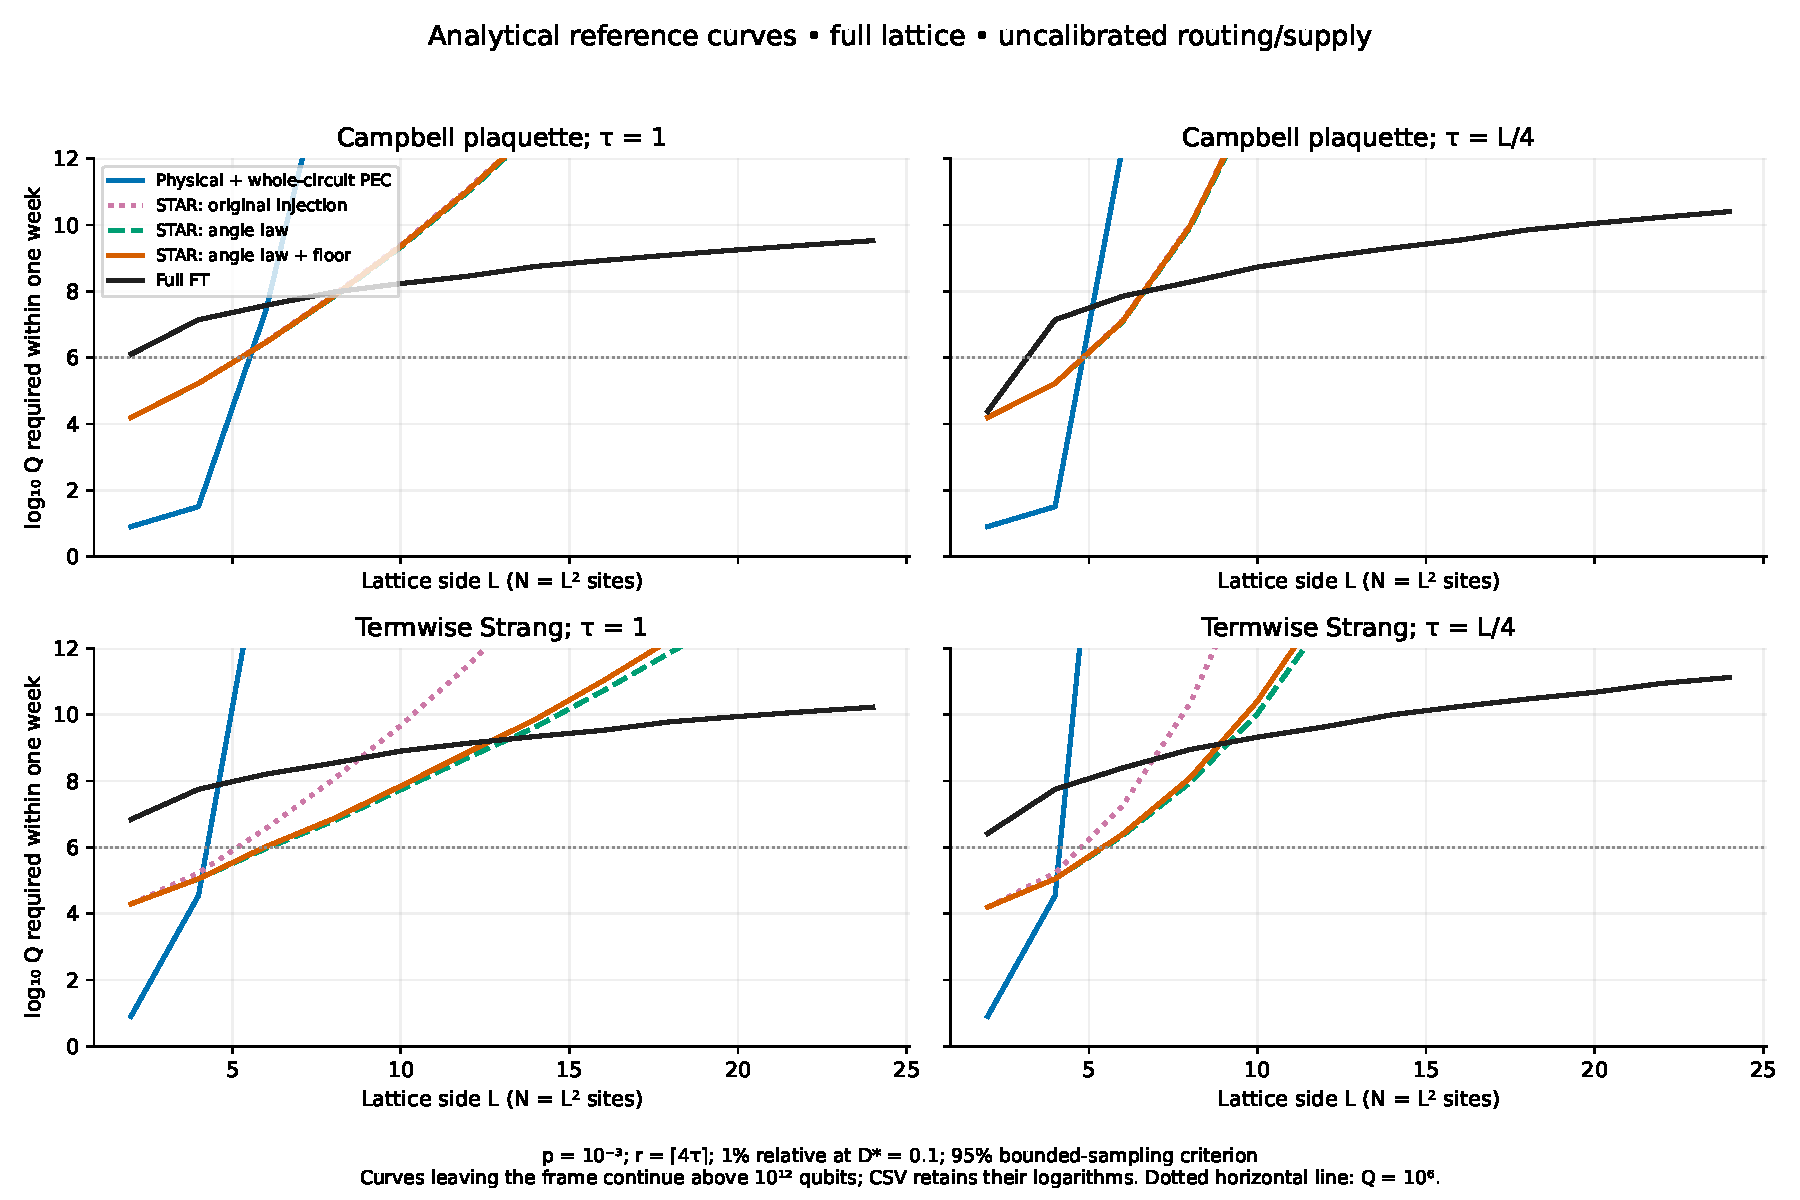
\includegraphics[width=\textwidth]{results/analytical_v1/first_scaling.pdf}
 \caption{Initial area estimates for completing the specified sampling task
 within one week, conditional on the shared step count and error budget.
 The two rows compare decompositions and the columns distinguish fixed time
 from system-scale time. Full-lattice execution is used throughout. Routing,
 injection supply, and syndrome suppression are reference assumptions; the
 curves locate mechanisms to investigate, not established device crossovers.}
 \label{fig:first}
\end{figure}
\begin{figure}[t]
 \centering
 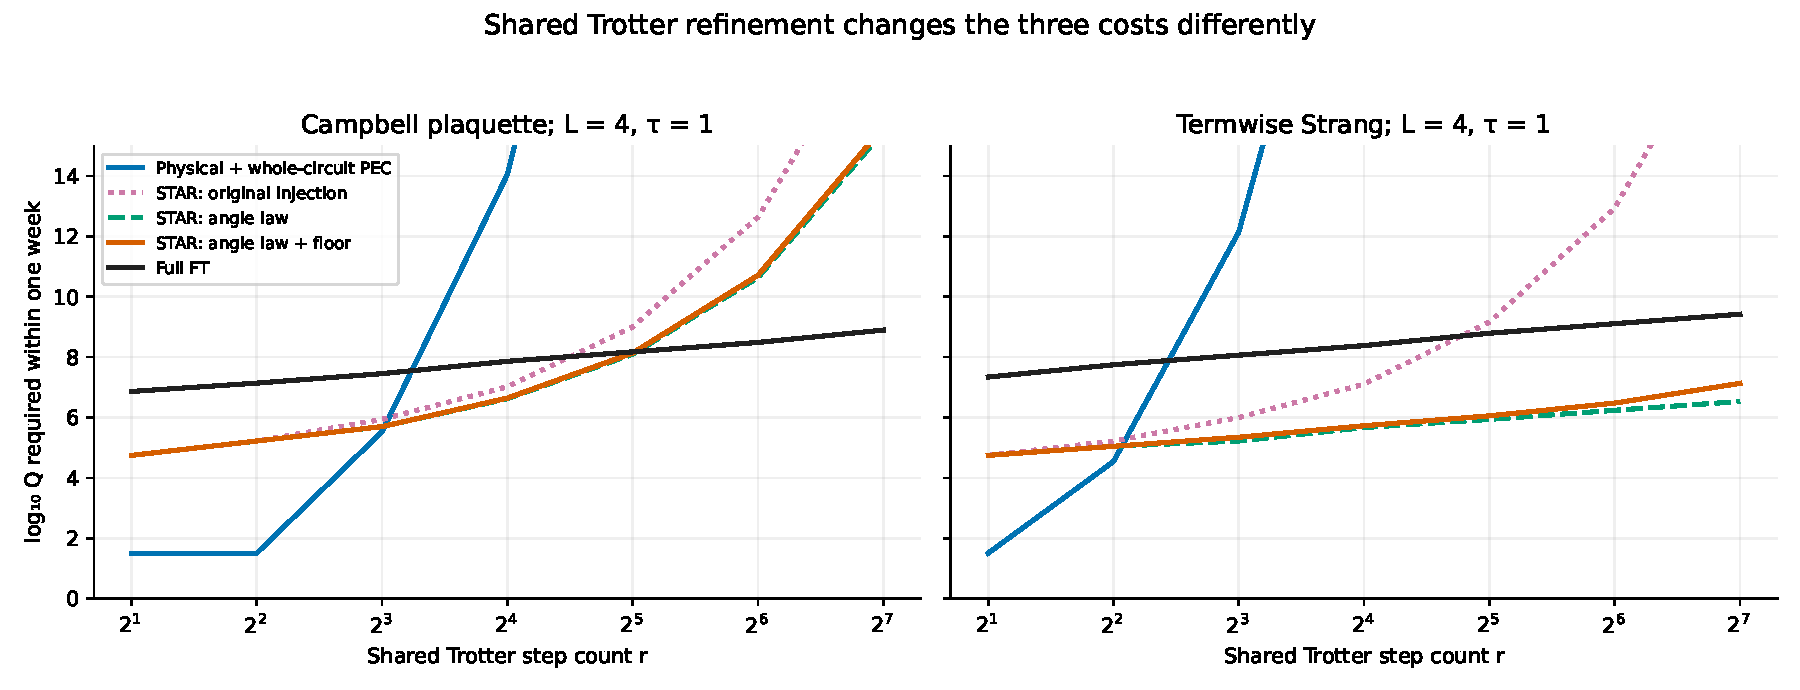
\includegraphics[width=\textwidth]{results/analytical_v1/step_sensitivity.pdf}
 \caption{Cost sensitivity to the same Trotter refinement at fixed $L$ and
 $\tau$. Physical PEC and original STAR pay per operation. In termwise
 small-angle STAR the leading angle exponent is invariant, while execution
 time and logical distance still change. Plaquette STAR also pays for repeated
 fixed-angle basis changes. Full FT grows through synthesis and execution.}
 \label{fig:steps}
\end{figure}

The central comparison is exponential exposure versus protected spacetime
volume. For termwise circuits with local compilation, $R=O(Nr)$ and
$\Theta=O(N\tau)$; thus physical PEC and original STAR have exponents
$O(pNr)$, while the small-angle term has exponent $O(pN\tau)$.
Full FT has $N_T=O(Nr\log(Nr/\eps))$ and logarithmic distance growth below
threshold. Plaquette compilation adds an $O(pNr)$ fixed-angle STAR term in
the present injection choice. These are conditional laws for the modeled
implementations, not exhaustive laws for the architectures.

The full-lattice curves at fixed $\tau$ should not be interpreted as the
optimal size dependence of a local observable. Physical truncation with
budgeted bias may make the required region saturate with $L$; exact circuit
cones and physical propagation regions are different objects. Both should
be offered to all three architectures when introduced.

For a proposed hybrid at fixed ideal shot budget, additional protection pays
when
\begin{equation}
 \Delta\log t_a+\Delta\log\Gamma^2-\Delta\log a-\Delta\log m<0.
\end{equation}
The repeated fixed gates in the plaquette construction give a concrete first
test: compare analog injection of all rotations with distilled fixed-angle
gates and analog small rotations, including the added supply and area.

\section{Refinement order and provenance}
The executable forms are in \texttt{model.py}; \texttt{assumptions.json}
contains every plotted numerical knob. \texttt{make\_plots.py} writes the
figures, logarithmic CSV data, sensitivities, and a source-hash manifest.
Tests verify inverse-channel coefficients by independent Pauli convolution,
term counts by explicit stage expansion, the open-boundary tile cover,
the plaquette spectrum, and logical-budget accounting. These checks validate
the calculation of the reference curves, not the device assumptions.

The next step is a common CUDA-Q Logical circuit with three compilation and
costing paths: native physical gates, protected Clifford gates with analog
rotations, and protected Clifford+$T$. Its output should replace the proxy
gate counts, routing, Clifford work, and timing while preserving the workload
and error conventions. The local CUDA-Q Hubbard implementation is controlled,
first order, and periodic by default; it cannot be substituted directly.
The built-in surface physical target is also a compact reference using native
multi-Pauli operations. STAR needs an explicit analog-rotation path.

Only after the first compiled comparison do we calibrate $r(\tau,\eps)$ for
the local observable, using analytical bounds and selected small-system
dynamics. Qubitization is deferred until this matched-algorithm baseline
is understood and remains a separately identified algorithm change.

\bibliographystyle{unsrt}
\bibliography{references}
\end{document}
